\chapter{Conexión por caminos}%
\label{cha:conexion_por_caminos}
\begin{defi}
Un \textbf{camino} en un espacio $X$ es una aplicación continua $\alpha: \left[ a, b \right] \subset \mathbb{R}_u \rightarrow X$. Decimos:
\begin{itemize}
    \item $\alpha$ \textbf{va de} $\alpha\left( a \right)$ a $\alpha\left( b \right)$, \textbf{conecta} $\alpha\left( a \right)$ con $\alpha\left( b \right)$, que son \textbf{extremos}.
    \item La imagen $\alpha\left[ a, b \right] \subset X$ es la \textbf{traza}, conexa por imagen continua.
\end{itemize}
\end{defi}

\begin{prop}[Cambios de parámetros]
$\forall \varphi: \left[ c, d \right] \rightarrow \left[ a, b \right]$ continua $\Rightarrow \beta = \alpha \circ \varphi$ es otro camino con igual traza.    

$\varphi$ es un \textbf{cambio de parámetro} cuando es homeomorfismo (creciente o decreciente).
\begin{figure}[H]
    \centering
    \incfig{cambio-de-caminos}
    \caption{\textit{Ejemplo de un cambio de parámetros para un camino.}}
    \label{fig:cambio-de-caminos}
\end{figure}
\end{prop}

\begin{ej}[Interpolación lineal]
Dados $p, q \in \mathbb{R}^n,\ \alpha : \left[ 0, 1 \right] \rightarrow \left[ p, q \right]: t \mapsto \left( 1 - t \right) p + tq$ es un camino bien conocido y útil. También sirve para reparametrizar si $\left[ p, q \right] = \left[ a, b \right] \subset \mathbb{R}$. Vemos, por ejemplo, que siempre podemos reducirnos a caminos con dominio $\left[ 0, 1 \right]$. Esto será fundamental más adelante. 
\end{ej}

\begin{prop}[Producto de caminos]
Topológicamente: 
\begin{figure}[H]
    \centering
    \incfig{producto-de-caminos}
    \caption{\textit{Ejemplo de un producto de caminos}}
    \label{fig:producto-de-caminos}
\end{figure}
(Alternativa: Reparametrizar $\beta$ con dominio $\left[ b, b + \left( d - c \right) \right]$)
\end{prop}

\begin{ej}
Si hacemos el producto de segmentos consecutivos obtenemos \textbf{caminos poligonales}. 
\end{ej}

\section{Conexión por caminos}%
\label{sec:conexion_por_caminos}
\begin{defi}
Un espacio $X$ es \textbf{conexo por caminos} si sus puntos se pueden conectar con un camino:
\[
\forall x \forall y \in X,\ \exists \sigma_y: \left[ a, b \right] \rightarrow X,\ \sigma_y\left( a \right) = x\; \land \;\sigma_y\left( b \right) = y
\]
\end{defi}
\begin{obs}
En particular, $X = \bigcup_{y \in X} \sigma_y\left[ a, b \right]$ es \underline{conexo} (pivote, $\alpha_y\left( a \right) = x,\ \forall y$)
\end{obs}

\begin{ej}
\begin{enumerate}
    \item La mayor parte de los conexos conocidos son conexos por caminos:
    \begin{itemize}
        \item Los abiertos conexos (top. usual) son conexos por poligonales, que son caminos.
        \item Los conjuntos convexos y los estrellados también.
    \end{itemize}
    \item El seno del topólogo $\Gamma$ es la traza de $\alpha\left( t \right) = \left( t, \sin\frac{1}{t} \right),\ t > 0$, es conexo y lo es su adherencia $\overline{\Gamma} = J \cup \Gamma,\ J = \{0\} \times \left[ 0, 1 \right]$. Pero $\overline{\Gamma}$ \underline{no} es conexo por caminos.
    \begin{demo}
        No existen caminos $\sigma: \left[ a, b \right] \rightarrow \overline{\Gamma} \begin{cases}
            \sigma\left( a \right) = p \in J\\
            \sigma\left( b \right) = q \in \Gamma
        \end{cases}$:
        \begin{figure}[H]
            \centering
            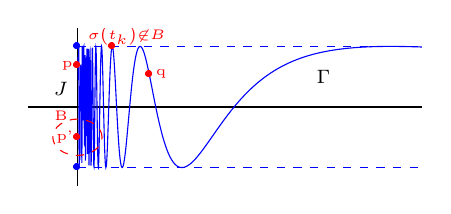
\begin{tikzpicture}
            \begin{axis}[
                axis lines* = middle,
                height=2cm,
                width=5cm,
                scale only axis=true,
                ytick=\empty,
                xtick=\empty,
                xmin=-0.1,
                xmax=0.7,
                ymin=-1.3,
                ymax=1.3,
            ]
            \addplot[
                domain=0.001:0.8,
                samples=1000,
                color=blue,
                smooth,
            ]
            {sin(deg(1/x))};
            \draw[blue, dashed] (0,1) -- (1,1);
            \draw[blue, dashed] (0,-1) -- (1,-1);
            \node at (0,0.3) [left] {\scriptsize $J$};
            \node[blue] at (0,1) {\tiny \textbullet};
            \node[blue] at (0,-1) {\tiny \textbullet};
 
            \node[red] at (0.01,0.68) [left] {\tiny p};
            \node[red] at (0,0.7) {\tiny \textbullet};

            \node[red] at (0.01,-0.5) [left] {\tiny p'};
            \node[red] at (0,-0.5) {\tiny \textbullet};

            \draw[red, dashed] (0,-0.5) ellipse (0.05 and 0.3);
            \node[red] at (0, -0.15) [left] {\tiny B};

            \node[red] at (0.071,1) {\tiny \textbullet};
            \node[red] at (0.1,0.85) [above] {$\scriptscriptstyle \sigma\left( t_k \right) \not\in B$};

            \node[red] at (0.146,0.55) {\tiny \textbullet};
            \node[red] at (0.14,0.55) [right] {\tiny q};

            \node at (0.5, 0.5) {\scriptsize $\Gamma$};
            \end{axis}
            \end{tikzpicture}
            \caption{\textit{La bola representada es de radio pequeño.}}
            \label{fig:seno_topologo_caminos}
        \end{figure}

        \begin{enumerate}
            \item $\sigma\left( t \right) = \left( \alpha\left( t \right), \beta\left( t \right) \right),\ \alpha, \beta$ continuas. $\exists a' = \max \{t \in \left[ a, b \right] : \alpha\left( t \right) = 0\} \Rightarrow (\alpha$ continua en un compacto) %TODO: Fix orden 
            $\Rightarrow \begin{cases}
                \alpha\left( a' \right) = 0,\ \sigma\left( a' \right) = p' \in J\\
                t > a': \alpha\left( t \right) > 0 \Rightarrow \sigma\left( t \right) \in \Gamma \Rightarrow \beta\left( t \right) = \sin \frac{1}{\alpha\left( t \right)} 
            \end{cases} $

            \item Supongamos $p' = \sigma\left( a' \right) \neq \left( 0, 1 \right)$ (punto) y $\exists \delta: B\left( p', \delta \right) \cap \{y = 1\} = \emptyset$. $\sigma$ continua $\Rightarrow \exists \sigma\left[ a', \varepsilon \right] \subset B\left( p', \delta \right) \Rightarrow \sigma\left[ a', \varepsilon \right] \cap \{y = 1\} = \emptyset$. (si $p' = \left( 0, 1 \right)$ evitaríamos $\{y = -1\}$)

            \item $\alpha$ continua $\Rightarrow \alpha\left[ a', \varepsilon \right] \subset \mathbb{R}$ conexo compacto $=$ intervalo: $\alpha\left[ a', \varepsilon \right] = \left[ 0, c \right]$.

            \item La oscilación de $\sin \frac{1}{x}$ lleva $\sigma$ a $\{y = 1\}$, fuera de la bola elegida:
            \begin{align*}
            k \gg 0 &\Rightarrow \frac{2}{\left( 1 + 4k \right) \pi} \in \left[ 0, c \right] = \alpha\left[ a', \varepsilon \right] \Rightarrow \exists a' < t_k < \varepsilon: \alpha\left( t_k \right) = \frac{2}{\left( 1 + 4k \right) \pi}\\ 
                &\Rightarrow \sigma\left( t_k \right) = \left( \alpha\left( t_k \right), \sin\left( \frac{1}{\alpha\left( t_k \right)} \right) \right) = \left( x_k, 1 \right) 
            \bot \end{align*}
        \end{enumerate}
    \end{demo}
\end{enumerate}
\end{ej}

\section{Mantras}%
\label{sec:mantras_conx_caminos}
Casi todo lo que dijimos sobre la conexión nos vale:
\begin{prop}[Mantra del pivote]
Sea $X = \bigcup_{i} A_i,\ \bigcap_{i} A_i \neq \emptyset,\ \forall A_i$ conexos por caminos $\Rightarrow X$ conexo por caminos. 
\end{prop}
\begin{demo}
Demostración por dibujo:
\begin{figure}[H]
    \centering
    \incfig[0.5]{teorema-del-pivote-caminos}
    \caption{\textit{Teorema del pivote con caminos}}
    \label{fig:teorema-del-pivote-caminos}
\end{figure}
\end{demo}

\begin{prop}[Mantra de la imagen]
Sea $f: X \rightarrow Y$ continua con $X$ conexo por caminos $\Rightarrow f\left( X \right)$ es conexo por caminos. 
\end{prop}
\begin{demo}
De nuevo, ilustramos la demostración con un dibujo:
\begin{figure}[H]
    \centering
    \incfig[0.4]{imagen-conexa-por-caminos}
    \caption{\textit{Imagen continua conexa por caminos}}
    \label{fig:imagen-conexa-por-caminos}
\end{figure}
\end{demo}

\begin{prop}[Mantra de la adherencia (¡NO!)]
El seno del topólogo $\Gamma$ es conexo por caminos: $\left( a, \sin\frac{1}{a} \right)$ y $\left( b, \sin\frac{1}{b} \right)$ se conectan por el camino evidente, $\alpha\left( t \right) = \left( t, \sin\frac{1}{t} \right),\ a \le t \le b$. Pero, como hemos visto, la adherencia $\overline{\Gamma}$ no es conexa por caminos. 
\end{prop}

\section{Tabla de comportamiento}%
\label{sec:tabla_de_comportamiento_conx_caminos}
%TODO: Fix tabla
\begin{table}[H]
\centering
\begin{tabular}{| c | c | c | c | c |}
\hline
& Subespacios & Cocientes & Productos & Sumas\\
\hline
Conexión por caminos & \ding{55} & \checkmark & \checkmark & \ding{55}\\
\hline
\end{tabular}
\caption{\textit{La tabla nos indica como se conserva la conexión por caminos en las construcciones que hemos visto. Las sumas y los productos son finitos.}}
\end{table}

\begin{prop}[Productos]
Sean $\left( x_1, y_1 \right),\ \left( x_2, y_2 \right) \in X \times Y$: 
\[
\begin{rcases}
    \sigma: \left[ a, b \right] \rightarrow X: \begin{cases}
        \sigma\left( a \right) = x_1\\
        \sigma\left( b \right) = x_2
    \end{cases}\\
    \tau: \left[ a, b \right] \rightarrow Y: \begin{cases}
        \tau\left( a \right) = y_1\\
        \tau\left( b \right) = y_2
    \end{cases}
\end{rcases} 
    \Rightarrow \gamma = \left( \sigma, \tau \right) : \left[ a, b \right] \rightarrow X \times Y: \begin{cases}
        \gamma\left( a \right) = \left( x_1, y_1 \right)\\
        \gamma\left( b \right) = \left( x_2, y_2 \right)
    \end{cases}  
\]
\end{prop}


\chapter{Componentes conexas\texorpdfstring{\\}{} por caminos y conexión\texorpdfstring{\\}{} local por caminos}%
\label{cha:componentes_conexas_por_caminos_y_conexion_local_por_caminos}
\section{Componentes conexas por caminos}%
\label{sec:componentes_conexas_por_caminos}
Todo análogo a las componentes conexas (casi). Sea $X$ espacio topológico.
\begin{defi}
Una \textbf{componente conexa por caminos} (c.c.c) es un subconjunto conexo por caminos maximal.
\end{defi}
\begin{prop}[Descripción]
\begin{enumerate}
    \item La c.c.c de $x \in X$ es $\bigcup_{x \in A} A$ con $A$ conexa por caminos.
    \item Las c.c.c forman una partición de $X$, más fina que la de las c.c.
    \begin{demo}
        Porque conexo por caminos $\Rightarrow$ conexo, pero no a la inversa.

        \textbf{¡OJO!} Las c.c.c no son necesariamente cerradas. 

        Como contraejemplo de ambas cosas dichas tenemos la adherencia del seno topólogo. 
    \end{demo}
\end{enumerate} 
\end{prop}

\begin{ej}
    $\Gamma$ seno del topólogo y $\overline{\Gamma} = J \cup \Gamma$ son conexos. Tenemos que $\overline{\Gamma}$ es una c.c, mientras que $J$ y $\Gamma$ son dos c.c.c, una cerrada ($J$) y la otra no ($\Gamma$). 
    \begin{demo}
    Porque $\overline{\Gamma}$ \underline{no} es conexa por caminos.
    \end{demo}
\end{ej}

\section{Conexión local por caminos}%
\label{sec:conexion_local_por_caminos}
Imitamos sin sorpresa las demostraciones de la conexión local y tenemos:
\begin{defi}
$X$ es \textbf{localmente conexo por caminos} si $\forall x \in X,\ \exists \mathcal{B}^x$ base de entornos abiertos conexos por caminos.
\end{defi}
\begin{prop}
$X$ es localmente conexo por caminos $\Leftrightarrow$ las c.c.c de un abierto son abiertas.
\end{prop}

\begin{enun}
Locamente conexo $\Leftrightarrow \forall x \in X,\ \exists \mathcal{V}^x$ base de entornos conexos por caminos. 
\end{enun}

\section{Tabla de comportamiento}%
\label{sec:tabla_de_comportamiento_conx_local_caminos}
%TODO: Fix tabla
\begin{table}[H]
\centering
\begin{tabular}{| c | c | c | c | c |}
\hline
& Subespacios & Cocientes & Productos & Sumas\\
\hline
Conexión local por caminos & \ding{55} & \checkmark & \checkmark & \checkmark\\
\hline
\end{tabular}
\caption{\textit{También vale que las c.c.c del producto son los productos de las c.c.c de los factores.}}
\end{table}

\section{Relaciones entre las propiedades de conexión}%
\label{sec:relaciones_entre_las_propiedades_de_conexion}
Lo principal es que:
\begin{prop}
Conexo y localmente conexo por caminos $\Rightarrow$ Conexo por caminos.
\end{prop}
\begin{demo}
\begin{itemize}
    \item Conexo $\Rightarrow \forall x, y,\ \exists \text{ cadenas de } x \text{ a } y$.
    \item Localmente conexo por caminos $\Rightarrow$ cadenas de abiertos conexos por caminos $\xRightarrow{\text{Variante del pivote}}$ Estas cadenas son conexas por caminos.
\end{itemize}
Por tanto, $\exists$ camino de $x$ a $y$.
\end{demo}
\begin{obs}
    Esta es la demostración de que un abierto conexo de $\mathbb{R}_u^n$ lo es por poligonales (se usan cadenas de bolas).
\end{obs}

\begin{obs}[Resumen]
Por especificar todas las posibilidades:
%TODO: Imagen
\begin{center}
    \includegraphics[scale=0.3]{images/resumen_conx} 
\end{center}
\end{obs}

\begin{enun}
Contraejemplos. Los menos fáciles son $*$ y $**$ 
\end{enun}

\begin{ej}
\begin{itemize}
    \item Sea $\left( \mathbb{R}^2, \mathcal{T}_{\text{rad}} \right)$. Veamos si es conexo por caminos porque entonces será conexo.

    %TODO: Dibujo
    Primero intentamos parametrizar por interpolación: $\left( 1 - t \right)a + tb$. Como $\mathcal{T}_{\text{rad}}|_r = \mathcal{T}_{u}|_r$ es correcto el camino ($r$ es una recta).
    En cambio si el camino es una curva cualquiera, la topología relativa es la discreta, es decir, la preimagen de un punto es todo $\left[ 0, 1 \right]$ al ser 
    un abierto y cerrado en un conexo. Por tanto, $f$ será constante (contradicción).

    En definitiva, tomamos como caminos entre dos puntos, la recta que los une. Con esto, el espacio es conexo por caminos $\Rightarrow$ conexo.

    La usual es localmente conexa por caminos. Si en la radial es localmente conexa por caminos tenemos que si $x_0 \in U$ entonces $\exists U \supset V_{\text{ab}} = C_{\text{cam.}} \left( x_0 \right)$es el candidato a entorno abierto conexo por caminos de la base buscada. 

    Usaremos $V = \left\{ x \in U : \exists P \supset U: x_0 \rightarrow x\right\}$ con $P$ poligonal %TODO: Dibujo
    que será conexo por caminos radiales. Veamos que es abierto (radial).

    Esto quiere decir que $\forall x \in V$ se cumple ``la condición radial''.
    %TODO: Dibujo
    $\exists \underbrace{\left( x - \varepsilon, x + \varepsilon \right)}_{\ni y} \subset U \cap L$. Formamos $P_y = P_x \cup \left[ x, y \right] \subset U \Rightarrow \left( x - \varepsilon, x + \varepsilon \right) \subset V \cap L$.

    %TODO: Cambiar de lugar
    \item Veamos ahora la compacidad tenemos que $\mathcal{T}_u \subset \mathcal{T}_r \Rightarrow$ si $K$ compacto en la radial $\Rightarrow$ también lo será en la usual. Por tanto, al no ser $\mathbb{R}^2$ con la usual compacto, tampoco lo será con la radial.

    En cambio como con la usual, $\mathbb{R}^2$ sí es Lindelöf no podemos decidir directamente si con la radial lo es o no. Pero no es así porque las curvas son cerradas pero su topología relativa es la 
    discreta y, por tanto, no son Lindelöf. Como se hereda, la radial no puede ser Lindelöf.

    \item Veamos la compacidad local. No lo es. %TODO: Imagen.
\end{itemize}
\end{ej}
